\chapter{Qubits}
\label{chap:qubits}

Un \gls{qubit} es el análogo cuántico al bit clásico \cite{ionos_qubits_2023}. Mientras el bit tiene \textbf{dos posibles estados}, el 0 y el 1, el \gls{qubit} se representa como un vector en el espacio vectorial $\mathbb{C}^2$. La base del espacio más utilizada, se denomina base computacional y se corresponde con la base canónica de $\mathbb{C}^2$, que en \textit{notación de Dirac}, son los vectores $\ket{0}$ y $\ket{1}$:

\begin{equation*}
    \begin{array}{rl}
        \ket{0} = & \begin{bmatrix}
                        1 \\ 0
                    \end{bmatrix} \in \mathbb{C}^2 \\
        \ket{1} = & \begin{bmatrix}
                        0 \\ 1
                    \end{bmatrix}
    \end{array}
\end{equation*}

\textbf{Un estado cuántico} es la descripción matemática completa de un sistema cuántico aislado (en este caso, un \gls{qubit}). Más allá de ser un simple vector, este estado encapsula toda la información física y probabilística que podemos conocer del sistema antes de interactuar con él. Dado que se define dentro de un espacio de Hilbert, el estado cuántico obedece al \textit{principio de superposición}, lo que le confiere la capacidad de existir en múltiples configuraciones clásicas de forma simultánea hasta que se produce el colapso mediante una medición.

\section{Expresión del Qubit en Superposición}
Gracias al principio de superposición mencionado anteriormente, un qubit $\ket{\Psi}$ no tiene por qué estar exclusivamente en el estado $\ket{0}$ o en el estado $\ket{1}$. En su lugar, su estado puede ser una \textbf{combinación lineal} de ambos vectores base. A este comportamiento se le denomina \textbf{superposición cuántica}, y permite que el qubit exista como una mezcla simultánea de ambos estados clásicos. En notación de Dirac, esto se representa algebraicamente como:

\[
    \ket{\Psi} = \alpha_0\ket{0} + \alpha_1\ket{1}
\]

Donde $\alpha_0$ y $\alpha_1$ son las \textbf{amplitudes de probabilidad}. De forma general, estas amplitudes se definen como números complejos (lo que, por definición matemática, también incluye a los números reales como un caso particular). Dado que estos coeficientes pueden tomar infinitos valores continuos, un qubit puede adoptar \textbf{infinitos} estados posibles, frente a los únicos dos valores (0 y 1) de un bit clásico. Para que este estado sea válido físicamente, su norma debe ser unitaria, asegurando que la suma de las probabilidades sea 1:

\[
    |\alpha_0|^2 + |\alpha_1|^2 = 1
\]

Cabe destacar que no existe una forma directa de determinar los valores exactos de $\alpha_0$ y $\alpha_1$, ya que el estado cuántico interno no es directamente observable. Antes de realizar una medición, el qubit se encuentra en esta superposición inestable de los estados $\ket{0}$ y $\ket{1}$.

Para conocer el resultado de una computación cuántica, es necesario medir los qubits \cite{sholtis_measure_qubits_2019}. Sin embargo, el acto de medición implica una interacción física que perturba irreversiblemente el sistema. Esto provoca que el qubit abandone su estado de superposición y experimente el \textbf{colapso}. Al colapsar, el qubit se ve forzado a tomar un único valor clásico definido, es decir, pasa a ser estrictamente un $0$ lógico (estado $\ket{0}$) o un $1$ lógico (estado $\ket{1}$). Una vez medido, el qubit se comporta como un bit clásico ordinario, y la información sobre sus amplitudes cuánticas originales se pierde de forma irrecuperable.

La probabilidad exacta de que el qubit colapse hacia un estado u otro está dictada por la \textbf{regla de Born}. Esta regla establece que la probabilidad de observar cada resultado clásico es igual al módulo al cuadrado de su amplitud correspondiente ($P(0) = |\alpha_0|^2$ y $P(1) = |\alpha_1|^2$).

La superposición, tiene distintas representaciones que son:

\begin{itemize}
    \item \textbf{Binómica:} $\ket{\Psi} = (x_0 + i y_0) \ket{0} + (x_1 + i y_1) \ket{1}$
    \item \textbf{Exponencial:} $\ket{\Psi} = r_0 e^{i\phi_0} \ket{0} + r_1 e^{i\phi_1} \ket{1}$
    \item \textbf{Senos y cosenos:} $\ket{\Psi} = \cos\left(\frac{\theta}{2}\right) \ket{0} + e^{i\phi} \sin\left(\frac{\theta}{2}\right) \ket{1}$
\end{itemize}

Existen otros dos conceptos fundamentales relacionados con la superposición y sus fases complejas:

\begin{itemize}
    \item \textbf{Fase global:} Factor común $e^{i\gamma}$ que multiplica a todo el estado $\ket{\Psi}$. Este no cambia ninguna probabilidad ni resultado físico.
    \item \textbf{Fase relativa:} Es la diferencia entre las amplitudes $\alpha$ y $\beta$. Esto influye a las inferencias y los resultados cuando se miden en otras bases $(X, Y)$.
\end{itemize}


\section{Esfera de Bloch}

La esfera de Bloch es una representación visual del estado de un qubit.
Cada punto sobre su superficie corresponde a una posible superposición de los estados base $\ket{0}$ y $\ket{1}$.
Los polos superior e inferior representan los estados $\ket{0}$ y $\ket{1}$, respectivamente, y el estado del qubit se indica con una flecha que apunta hacia el punto que lo describe.

\begin{comment}
\begin{figure}[h]
    \centering
    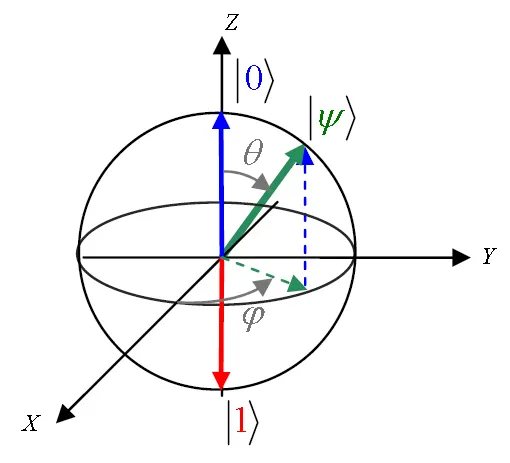
\includegraphics[width=0.5\linewidth]{imagenes/EsferaDeBloch.png}
    \caption{Visualización gráfica esfera de Bloch}
    \label{fig:EsferaDeBloch}
\end{figure}
\newpage

La representación de la esfera de Bloch de la imgaen, se le conoce como \textbf{ejes de Pauli}. Como tiene ángulos, se utiliza la representación de coordenadas esféricas principalmente. En dicha representación, se proporciona los dos ángulos y la longitud que viene denotado como $(r, \theta,\phi)$
donde $r$ es la longitud y $\theta$ y $\phi$ representan el ángulo del eje Z positivo con el de X positivo en el plano X-Z y el angulo entre el eje positivo X y el eje positivo Y del plano X-Y respectivamente
\end{comment}

\begin{figure}[h]
    \centering
    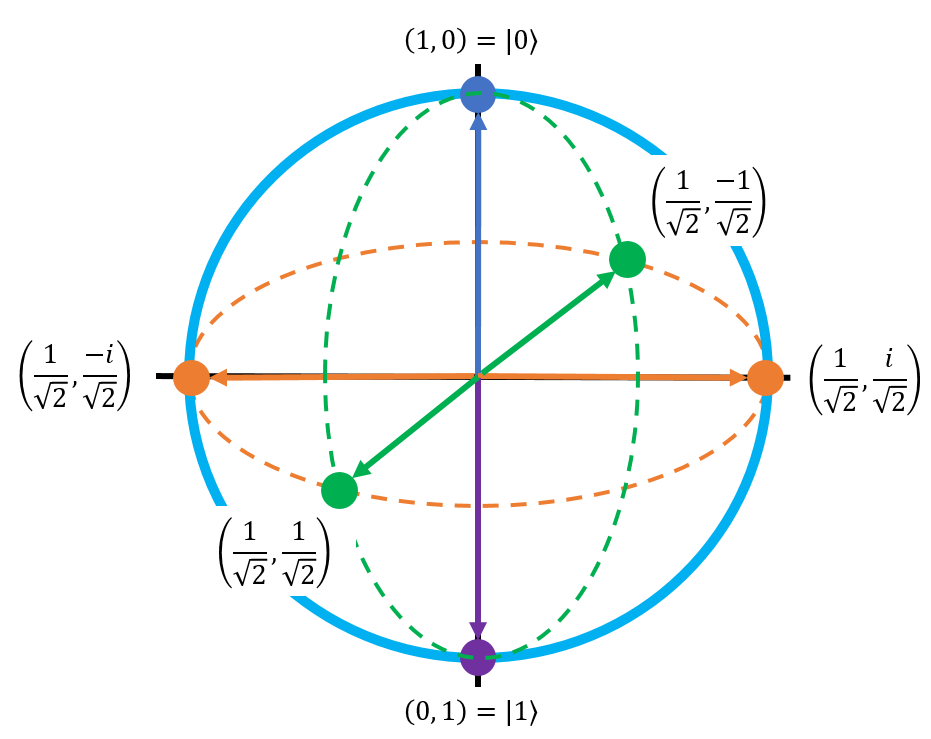
\includegraphics[width=0.5\linewidth]{imagenes/bloch-basic.png}
    \caption{Visualización gráfica de la esfera de Bloch. Imagen obtenida de \cite{mitre_bloch_sphere_2022}}
    \label{fig:EsferaDeBloch}
\end{figure}
\newpage

\textbf{Importante:} la notación $\left(\frac{1}{\sqrt{2}}, \frac{1}{\sqrt{2}}\right)$ se corresponde con el vector estado $\begin{bmatrix} \frac{1}{\sqrt{2}} \\ \frac{1}{\sqrt{2}} \end{bmatrix}$ que a su vez significa:

\[
    \begin{bmatrix} \frac{1}{\sqrt{2}} \\ \frac{1}{\sqrt{2}} \end{bmatrix} = \frac{1}{\sqrt{2}}|0\rangle + \frac{1}{\sqrt{2}}|1\rangle
\]

Los seis puntos principales de la esfera de Bloch son los que se ve en la Figura \ref{fig:EsferaDeBloch} \cite{castano_qubit_bloch_2025}. A estas coordenadas principales se le pueden asignar etiquetas.

\begin{itemize}
    \item \textbf{Base de Hadamard:} También se le conoce como eje X de Pauli. El punto $\left(\frac{1}{\sqrt{2}}, \frac{1}{\sqrt{2}}\right)$ se corresponde con $\ket{+}$. A su vez, el punto opuesto $\left(\frac{1}{\sqrt{2}}, \frac{-1}{\sqrt{2}}\right)$ se corresponde con $\ket{-}$

    \item \textbf{Base circular:} También se le conoce como eje Y de Pauli. El punto $\left(\frac{1}{\sqrt{2}}, \frac{i}{\sqrt{2}}\right)$ se corresponde con $\ket{+i}$. A su vez, el punto opuesto $\left(\frac{1}{\sqrt{2}}, \frac{-i}{\sqrt{2}}\right)$ se corresponde con $\ket{-i}$
\end{itemize}

Con dicha asignación de etiquetas, queda la esfera que se muestra en la Figura \ref{fig:EsferaDeBlochReducido}:

\begin{figure}[h]
    \centering
    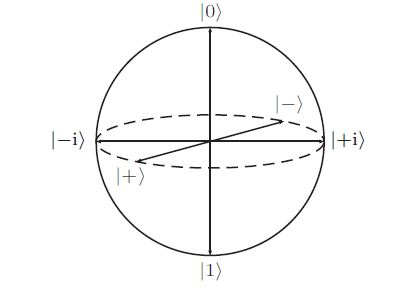
\includegraphics[width=0.5\linewidth]{imagenes/bloch-labels.jpg}
    \caption{Imagen obtenida de \url{https://en.wikipedia.org/wiki/Bloch_sphere}}
    \label{fig:EsferaDeBlochReducido}
\end{figure}
\newpage

\section{Puertas cuánticas}

Al igual que para manipular los valores de los bits existen puertas lógicas clásicas como OR, AND, NOT, etc. Los ordenadores cuánticos manipulan los valores de los qubits usando puertas cuánticas \cite{spinq_quantum_gates_2025}. Esto implica que cualquier algoritmo cuántico se tiene que implementar usando puertas cuánticas.

Las puertas cuánticas se \textbf{representan} matemáticamente mediante \textbf{matrices unitarias} $U$ \cite{gopalan_module3_2022}. Una matriz se considera unitaria si, al multiplicarla por su adjunta o conjugada transpuesta ($U^{\dagger}$), el resultado es la matriz identidad ($U^{\dagger}U = U U^{\dagger} = I$). Esta propiedad matemática es fundamental porque garantiza que la transformación es \textbf{reversible} y preserva la norma de los vectores. Esto significa que la puerta cuántica conserva siempre la probabilidad total de todos los posibles resultados, por lo que no se destruye ni se pierde información cuántica durante la operación.

Al aplicar una puerta cuántica $U$ a un estado cuántico $\ket{\psi}$ se realiza la multiplicación matricial $\ket{\psi'} = U \ket{\psi}$. Si expresamos el nuevo estado resultante como $\ket{\psi'} = \alpha_0' \ket{0} + \alpha_1' \ket{1}$, la propiedad unitaria asegura que la norma siga siendo unitaria. Es decir, independientemente de la puerta cuántica que se aplique, la regla de conservación de probabilidad se mantiene intacta: $|\alpha_0'|^2 + |\alpha_1'|^2 = 1$.

Poniendo un ejemplo sencillo, consideremos la puerta Pauli-X (el análogo cuántico de la puerta NOT clásica), cuya matriz unitaria es $X = \begin{pmatrix} 0 & 1 \\ 1 & 0 \end{pmatrix}$. Si aplicamos esta puerta sobre el estado base $\ket{0}$, el estado transiciona a $\ket{1}$:

\[
    X \ket{0} = \begin{pmatrix} 0 & 1 \\ 1 & 0 \end{pmatrix} \begin{pmatrix} 1 \\ 0 \end{pmatrix} = \begin{pmatrix} 0 \\ 1 \end{pmatrix} = \ket{1}
\]

Como $X$ es una matriz unitaria (y resulta ser su propia inversa, $X^{\dagger}X = I$), la operación es completamente reversible. Si aplicamos $X$ por segunda vez, recuperamos matemáticamente el estado original $\ket{0}$ sin perder ninguna información en el proceso:

\[
    X (X \ket{0}) = X \ket{1} = \begin{pmatrix} 0 & 1 \\ 1 & 0 \end{pmatrix} \begin{pmatrix} 0 \\ 1 \end{pmatrix} = \begin{pmatrix} 1 \\ 0 \end{pmatrix} = \ket{0}
\]

Las puertas cuánticas para un único qubit son:

\begin{itemize}
    \item \textbf{Pauli I (Identidad):} Se considera la operación trivial o identidad. Su función es dejar el qubit inalterado, y su operador asociado se denota mediante la matriz identidad $I$:
          \[
              I = \begin{bmatrix}
                  1 & 0 \\
                  0 & 1
              \end{bmatrix}
          \]

    \item \textbf{Pauli X:} Conocida coloquialmente como la puerta NOT cuántica. Algebraicamente se define por la siguiente matriz:
          \[
              X = \begin{bmatrix}
                  0 & 1 \\
                  1 & 0
              \end{bmatrix}
          \]

          Al aplicar esta puerta, las amplitudes de probabilidad se intercambian, lo que provoca que los estados base $\ket{0}$ y $\ket{1}$ se inviertan.

    \item \textbf{Pauli Y:} Esta transformación combina una inversión de los estados con un cambio de fase complejo. Su estructura viene dada por:
          \[
              Y = \begin{bmatrix}
                  0 & -i \\
                  i & 0
              \end{bmatrix}
          \]

          Si un qubit en superposición $\ket{\psi} = \alpha_0\ket{0} + \alpha_1\ket{1}$ atraviesa esta puerta, el efecto resultante es:
          \[
              Y\ket{\psi} = \begin{bmatrix} 0 & -i \\ i & 0 \end{bmatrix} \begin{bmatrix} \alpha_0 \\ \alpha_1 \end{bmatrix} = \begin{bmatrix} -i\alpha_1 \\ i\alpha_0 \end{bmatrix} = -i\alpha_1\ket{0} + i\alpha_0\ket{1}
          \]

    \item \textbf{Pauli Z:} Actúa modificando únicamente la fase del estado $\ket{1}$ (añadiendo un desfase de $\pi$). Su operador matricial se expresa como:
          \[
              Z = \begin{bmatrix}
                  1 & 0  \\
                  0 & -1
              \end{bmatrix}
          \]

          Matemáticamente, al operar sobre un qubit genérico $\ket{\psi} = \alpha_0\ket{0} + \alpha_1\ket{1}$, altera exclusivamente el signo de la segunda amplitud:
          \[
              Z\ket{\psi} = \begin{bmatrix} 1 & 0 \\ 0 & -1 \end{bmatrix} \begin{bmatrix} \alpha_0 \\ \alpha_1 \end{bmatrix} = \begin{bmatrix} \alpha_0 \\ -\alpha_1 \end{bmatrix} = \alpha_0\ket{0} - \alpha_1\ket{1}
          \]

    \item \textbf{Puerta Hadamard (H):} Es una de las operaciones más fundamentales, ya que al aplicarse sobre un estado base puro genera una superposición equitativa. Se define matricialmente como:
          \[
              H = \frac{1}{\sqrt{2}}\begin{bmatrix}
                  1 & 1  \\
                  1 & -1
              \end{bmatrix}
          \]

          Si aplicamos esta transformación a un estado en superposición $\ket{\psi} = \alpha_0\ket{0} + \alpha_1\ket{1}$, las amplitudes se mezclan obteniendo la siguiente salida:
          \[
              H\ket{\psi} = \frac{1}{\sqrt{2}}\begin{bmatrix} 1 & 1 \\ 1 & -1 \end{bmatrix} \begin{bmatrix} \alpha_0 \\ \alpha_1 \end{bmatrix} = \frac{1}{\sqrt{2}}\begin{bmatrix} \alpha_0 + \alpha_1 \\ \alpha_0 - \alpha_1 \end{bmatrix} = \left(\frac{\alpha_0 + \alpha_1}{\sqrt{2}}\right)\ket{0} + \left(\frac{\alpha_0 - \alpha_1}{\sqrt{2}}\right)\ket{1}
          \]
\end{itemize}